\documentclass[11pt]{article}
\usepackage{efavanzados}

\title{Elementos finitos avanzados}
\author{J. Rafael Rodríguez Galván}
\date{Marzo 2021}


\begin{document}
\maketitle
\tableofcontents

\subsection*{Prólogo}
En este documento se recogen una guía (incluyendo algunas anotaciones,
bibligrafía, etc.) para el curso de doctorado «Elementos finitos
avanzados» programado para el curso 2020/2021 en el Programa de
Doctorado en Matemáticas de la Universidad de Cádiz.

Los contenidos, resumidos en el siguiente índice, son muy ambiciosos y
deben verse como una lista de puntos de partida hacia muchas de las
áreas más avanzadas (rozando a la investigación) sobre análisis
numérico y resolución numérica de EDP mediante el método de los
elementos finitos y variantes cercanas a el. Haciendo énfasis no sólo
en su análisis teórico, sino en el manejo de algunos de los lenguajes,
bibliotecas y herramientas informáticas más relevantes.

Por supuesto, en un curso de estas características sería imposible
profundizar en todos ellos. La finalidad de este curso, menos
ambiciosa pero no menos motivadora, es realizar una aproximación
genérica a las materias aquí recogidas para, según las preferencias de
los estudiantes, poder profundizar en algunas de ellas.  Abrir las
puertas a la curiosidad, a investigar, estudiar, analizar, programar
ordenadores. Entorno a algunos de los aspectos más interesantes del
análisis y la simulación numérica de modelos de las ciencias experimentales.

Para este curso se presuponen una serie de conocimientos mínimos tanto
teóricos (por ejemplo, método de los elementos finitos) como prácticos
(conocimientos básicos de los lenguajes Python y C).



%==================================================
\section{Introducción}
%==================================================

\begin{contenidos}
  Introducción a la «shell» en entornos Unix. Sistemas
  de control de versiones. Lenguaje de programación
  Python. Introducción al entorno de elementos finitos
  FEniCS.
\end{contenidos}

\subsection{Introducción a la «shell» en entornos Unix}
\label{sec:intr-la-shell}

El objetivo de esta sección es familiarizarse con: algunos de los
conceptos básicos de la \textit{shell} UNIX, que serán útiles para el
resto de los temas. En concreto:
\begin{itemize}
\item Órdenes básicas de la \textit{shell}
\item Introducción a la programación de \textit{scripts}
\end{itemize}

Nos centramos en la \textit{shell Bash}, la más extendida\footnote{Por
  supuesto existen muchas otras \textit{shells} UNIX, entre ellas
  destacamos a \href{https://www.zsh.org/}{Zsh}} en entornos
UNIX. Como punto de partida, se puede utilizar alguna de las numerosas
guías o «reference cards» disponibles en internet, por ejemplo:
\begin{itemize}
\item \href{https://www.cs.jhu.edu/~joanne/unixRC.pdf}{UNIX (shell) reference card}
\item \href{http://web.mit.edu/merolish/Public/vi-ref.pdf}{Vi refference card}
\item \href{https://www.gnu.org/software/emacs/refcards/pdf/refcard.pdf}{Emacs refference card}
\end{itemize}

Las dos últimas referencias se centran en los editores \textit{VI} y
\textit{Emacs}, disponibles en terminales UNIX y también en entornos
gráficos de ventanas, con menús, botones etc (especialmente,
\textit{Emacs}). \textit{VI} (o \textit{VIM}, una versión «mejorada»)
es especialmente ubicuo en sistemas UNIX.

En la literatura existe bastante documentación sobre el manejo de la
\textit{shell}, abarcando desde el manejo básico de la consola hasta
la programación de \textit{scripts}. Aquí citamos por ejemplo dos
libros de la editorial O'Reilly~\cite{Newham-bash,Albing-Vosen-Bash},
que, en versión PDF, están disponibles en internet%
\footnote{Los libros se pueden descargar en formato PDF,
  respectivamente, de:
  \begin{itemize}
  \item \url{https://doc.lagout.org/operating\%20system\%20/linux/Learning\%20the\%20bash\%20Shell\%20-\%20Unix\%20Shell\%20Programming.pdf}
  \item \url{http://index-of.es/Programming/Bash/O\%27Reilly\%20bash\%20CookBook.pdf}
  \end{itemize}
  }.

\subsection{Sistemas de control de versiones}
Los sistemas de control de versiones permiten gestionar los cambios que se realizan en ficheros (usualmente, código fuente de programas, documentos \LaTeX, etc.). Este tipo de sistemas está diseñado para almacenar los ficheros, mantener un histórico de las acciones realizadas sobre ellos y facilitar la colaboración de distintas personas en su edición. En la actualidad, el más utilizado es el sistema de control de versiones \href{https://git-scm.com/}{Git}. Los ficheros y los cambios realizados se pueden almacenar en distintos \textit{repositorios}, locales o remotos. Existen algunos sitios web para almacenar repositorios remotos, públicos o privados: \href{https://github.com}{Github}, \href{https://gitlab.com/}{Gitlab}, \href{https://bitbucket.org}{Bitbucket}...

Como introducción y punto de entrada a Git se recomienda seguir alguno de los tutoriales disponibles en internet, por ejemplo \url{https://swcarpentry.github.io/git-novice/}. De nuevo, entre la abundante literatura sobre el tema, destacamos aquí una referencia de la que podemos descargar una versión en formato PDF\footnote{\url{https://gitlab.atica.um.es/palazon.um.es/gitParaTodos/blob/50ade3c49f78bd372e0237530c9abf27afb5dd0d/bib/O\%27Reilly\%20Git\%20Pocket\%20Guide\%202013.pdf}}.

\subsection{Lenguaje de programación Python}
\label{sec:python}


Python es un un lenguaje de programación\ldots{}
\begin{itemize}
\item De alto nivel\footnote{``Cercano al lenguaje
    natural'' (en este caso, al inglés), a diferencia de
    ``lenguajes máquina''.}.
\item De propósito general\footnote{En el sentido de estar orientado a
    su uso para numerosos fines: desde programación de aplicaciones para
    sistemas operativos hasta, juegos, proceso de audio, cálculo
    científico, móviles\ldots{}}.
\item Interpretado\footnote{Es decir, existe un programa (el
    \emph{intérprete}) que lee y ejecuta los programas sin necesidad
    de un proceso previo de compilación.}. Como tal, tiene sus ventajas
  (se agiliza el ciclo de desarrollo de software) e inconvenientes
  (menos rápido que los lenguajes compilados).
\item Orientado al \emph{desarrollo rápido} y a la legibilidad de los programas.
\item Cuenta con extensiones (bibliotecas) que lo convierten en una
      potente herramienta en el \emph{cálculo numérico} y científico.
    \item Muy \emph{popular} entre los desarrolladores de software, en
      general. En la actualidad, ocupa la primera plaza en numerosas
      clasificaciones\footnote{Basta echar un vistazo a \href{https://www.google.com/search?channel=fs&client=ubuntu&q=lenguajes+de+ordenador+m\%C3\%A1s+usados}{Google: lenguajes de ordenador más usados}}.
    \item Por último, pero : con \emph{licencia libre},
  disponible en las arquitecturas habituales \emph{Windows},
  \emph{Mac}, \emph{Linux}.
\end{itemize}

Python abre un gran abanico de posibilidades para quienes estén
interesados la informática, el cálculo numérico y científico. En este
curso se presuponen conocimientos mínimos en este lenguaje, así como
en editores (como \textit{Atom}, \textit{Spider}, o \textit{Emacs}),
entornos de desarrollo (como \textit{Jupyter}) y bibliotecas
matemáticas (\textit{numpy}, \textit{matplotlib}...)
especializados. De nuevo, existe una numerosa bibliografía y recursos
disponibles en internet.

%%% Local Variables:
%%% mode: latex
%%% TeX-master: "efavanzados.tex"
%%% End:


\section{El lenguaje C++}

\begin{contenidos}
  El lenguaje de programación C++. Programación orientada a
  objetos. Implementación de bibliotecas de elementos finitos.
\end{contenidos}



%%% Local Variables:
%%% mode: latex
%%% TeX-master: "efavanzados.tex"
%%% End:

\newcommand{\mfem}{\textit{MFEM}\xspace}
\newcommand{\glvis}{\textit{GLVis}\xspace}

\section{La biblioteca de elementos finitos \mfem. Problemas de evolución. Sistemas de EDP}
\subsection{Instalación}
\label{sec:03:instalacion}

\mfem \url{https://mfem.org} es «una biblioteca C++ gratuita, liviana
y escalable para métodos de elementos finitos».  Entre sus
características, descritas en \url{https://mfem.org/features}:
elementos 2D y 3D en triángulos, cuadriláteros, hexaedros, etc., orden
alto, $H^1$--conformes o $L^2$--discontinuos, elementos isogeométricos
(NURBS)...  Como todas las herramientas que se describirán a
continuación \mfem tiene licencia libre.

Aunque, como se puede comprobar en la web
\url{https://mfem.org/building/} existen versiones precompiladas que
usan sistemas de paquetes como \textit{Spack}, optaremos por la
instalación manual a partir de la compilación del código fuente.
Esto será más complicado, pero una vez sepamos hacerlo tendremos una
versión de la biblioteca expresamente compilada para nuestro sistema
y, en el futuro, tendremos garantizado el disponer de la última
versión, siempre que descarguemos las fuentes y volvamos a compilar.

Para ello, empezamos por descargar y descomprimir en una carpeta de
nuestro ordenador el archivo\footnote{Este tipo de archivos, de tipo
  \textit{.tar} y comprimidos con \texttt{gzip}, se usan desde hace
  décadas en sistemas UNIX.}  \texttt{.tgz} de su web,
\url{https://mfem.org/}.
\begin{itemize}
\item Esta será la última versión ``estable'' disponible del \textbf{código fuente de MFEM}.
\item De forma alternativa, se puede descargar la última versión ``inestable''de Github
\end{itemize}


A continuación, seguiremos las instrucciones del archivo
\href{https://raw.githubusercontent.com/mfem/mfem/master/INSTALL}{\textit{INSTALL}},
disponible en la web o en la carpeta donde descomprimimos anteriormente el código.

Comenzaremos por compilar una \textbf{versión secuencial} de \mfem. Más
adelante, hablaremos de la versión paralela. Los prerequisitos son:
\begin{itemize}
\item Un compilador de C++11, por ejemplo GCC.
\item Se recomienda disponer de una instalación de la biblioteca
  \textit{\glvis} para la visualización interactiva de mallas y
  funciones definidas sobre ellas.
\end{itemize}

Para la compilación suponemos además que se dispone de
\begin{itemize}
\item \textit{Make}
\item \textit{CMake}
\end{itemize}

\begin{lstlisting}[language=sh]
$ mkdir build
$ cd build
$ cmake ..
$ make -j 4
\end{lstlisting}

\begin{itemize}
\item En lo anterior, \texttt{build} es el nombre del directorio que
  elijamos para la compilación y \texttt{4} es el número de hilos
  paralelos durante el proceso de compilación.

\item \textit{CMake} es una
  herramienta de generación de código. Se ocupa de estudiar la
  disponibilidad en nuestro ordenador de las bibliotecas y otras
  herramientas necesarias para la compilación y, con esta información,
  genera un fichero \texttt{Makefile}.

\item Este fichero contiene las órdenes efectivas para la compilación
  y es utilizado (en la línea 4) por \textit{Make}, entorno de más
  bajo nivel que \textit{CMake}, para realizar este proceso y generar
  el código binario de \mfem.
\end{itemize}

Cuando finaliza la compilación, podemos ejecutar un primer test para
ver que la \mfem funciona correctamente ejecutando:
\begin{lstlisting}[language=sh]
$ make check
\end{lstlisting}
Esta orden compila y ejecuta el
\href{https://github.com/mfem/mfem/blob/master/examples/ex1.cpp}{ejemplo
  1} de la documentación de \mfem (ver
\url{https://mfem.org/examples}), que resuelve un problema para el
operador Laplaciano con condiciones de contorno Dirichlet.
\begin{lstlisting}
$ make check
[  0%] Built target copy_data
[  0%] Built target exec_prerequisites
[ 97%] Built target mfem
[100%] Built target ex1
Test project /home/rrgalvan/src/mfem/mfem-4.2/build
    Start 4: ex1_ser
1/1 Test #4: ex1_ser ..........................   Passed    0.15 sec

100% tests passed, 0 tests failed out of 1

Total Test time (real) =   0.15 sec
[100%] Built target check
\end{lstlisting}


Cuando finaliza la compilación, tendremos en nuestro directorio el fichero binario que contiene la biblioteca \mfem (por ejemplo, en sistemas GNU/Linux, el fichero \verb|libmfem.a|.


\subsection{El visualizador \glvis}
\label{sec:glvis}

Antes de su instalación, debemos asegurarnos de tener instalados los
paquetes que \glvis necesita. Esto varía en función del sistema
operativo (ver \url{https://glvis.org/building}).
Por ejemplo, en sistemas GNU/Linux derivados de la distribución \textit{Debian}, como \textit{Ubuntu}:
\begin{lstlisting}[language=sh]
$ apt-get install libfontconfig1-dev libfreetype-dev libsdl2-dev libglew-dev libglm-dev libpng-dev
\end{lstlisting}

Una vez contamos con los paquetes necesarios, podemos compilar, por
ejemplo usando directamente \textit{Make}. Será necesario indicar (en
la variable \verb|MFEM_dir|), el directorio donde, previamente, hemos
realizado la instalación de \mfem.
\begin{lstlisting}[language=sh]
$ make MFEM_DIR=../mfem-4.2/build -j 4
\end{lstlisting}

En este momento, podemos ejecutar \glvis, que queda a la espera de que
\mfem (u otro programa) le envíe datos para ser visualizados:
\begin{lstlisting}
$ ./glvis

       _/_/_/  _/      _/      _/  _/
    _/        _/      _/      _/        _/_/_/
   _/  _/_/  _/      _/      _/  _/  _/_/
  _/    _/  _/        _/  _/    _/      _/_/
   _/_/_/  _/_/_/_/    _/      _/  _/_/_/

Waiting for data on port 19916 ...
\end{lstlisting}
% $

Para hacer una prueba, abrimos otra terminal\footnote{O, en la misma
  terminal, pasamos \glvis a modo \textit{background} (pulsamos
  \texttt{Control+Z} y tecleamos \texttt{bg}).}. A continuación, nos
situamos en la carpeta \texttt{build/examples} (asumiendo que
\texttt{build} es el directorio de compilación de \mfem) y ejecutamos el ejemplo 1. Se obtendrá una representación gráfica similar a la mostrada en la figura

\begin{figure}
  \centering
  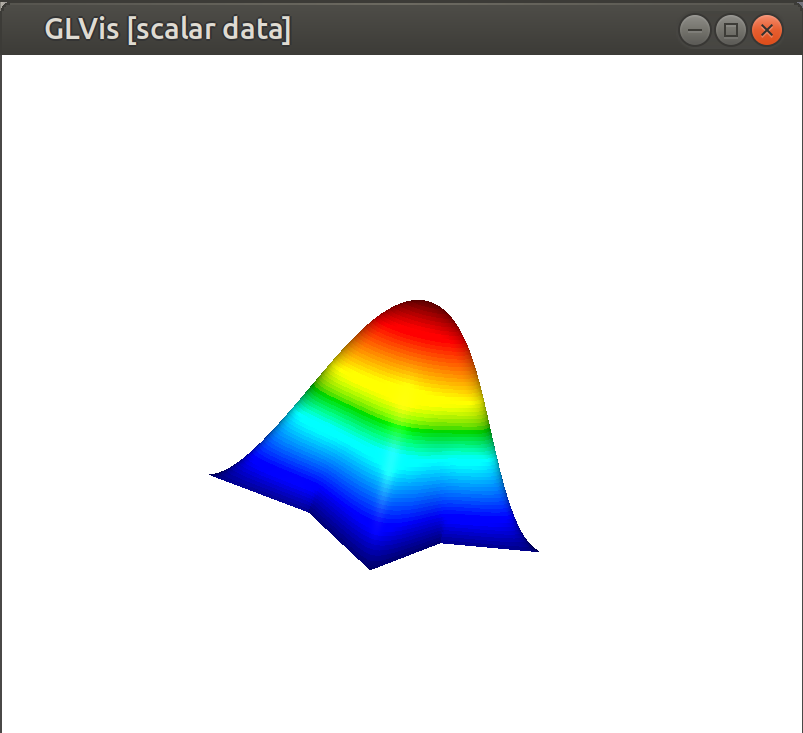
\includegraphics[width=0.3\linewidth]{img/ex1-glvis}
  \caption{Gráfica del ejemplo 1 de MFEM, visualizada con GLVis}
  \label{fig:ex1-glvis}
\end{figure}

Podemos modificar la visualización utilizando el ratón o alguna de las
combinaciones de tecla que se describen en el fichero
\href{https://raw.githubusercontent.com/glvis/glvis/master/README}{\textit{README}}. Por
ejemplo, podemos utilizar la tecla \texttt{m} para elegir la forma de
visualización de la malla, \texttt{S} para guardar\footnote{El fichero
  gráfico estará en el directorio desde donde se ejecutó el servidor
  de \glvis y su nombre será del tipo \texttt{GLVis\_s01.png}} una
captura de pantalla (\textit{snapshot}) y la tecla \texttt{q} para
salir (\textit{quit)}.


\subsection{Un primer ejemplo con \mfem}
\label{sec:3:un-primer-ejemplo}

\mfem se ha diseñado como una biblioteca C++ cuya jerarquía de clases
proporciona una serie de bloques básicos para desarrollar algoritmos
de tipo elementos finitos. Estos bloques básicos se describen
brevemente en \url{https://mfem.org/fem}. La jerarquía de clases se
describe por completo en la página web de
\href{https://mfem.github.io/doxygen/html/index.html}{documentación
  del código C++}\footnote{Esta página es generada automáticamente a
  partir de los comentarios incluidos en el código fuente, utilizando
  \href{https://www.doxygen.nl/index.html}{Doxygen}, una excelente
  herramienta para documentación en C++ (y otros lenguajes)} de \mfem.

Para comenzar a familiarizarse con la biblioteca \mfem, es
recomendable comenzar por el estudio de los ejemplos «canónicos»
disponibles en \url{https://mfem.org/examples/} y en el subdirectorio
\texttt{examples} del código fuente de \mfem.

Estudiaremos a continuación el
\href{https://github.com/mfem/mfem/blob/master/examples/ex1.cpp}{ejemplo
  1} de la documentación. Atendiendo a los comentarios insertados en
el código fuente, este ejemplo se divide en los siguientes apartados:
\begin{enumerate}
\item Analizar las «opciones», parámetros que pueden ser
  recibidos eventualmente desde la línea de comandos.
\item Habilitar, optativamente, dispositivos de hardware, como GPU, y
  modelos de programación, como CUDA u OpenMP.
\item Leer de un archivo la \textbf{malla} (formada por triángulos,
  cuadriláteros, hexaedros, ...).
\item Refinar (uniformemente) la malla hasta la resolución deseada.
\item Definir un \textbf{espacio de elementos finitos}.
\item Determinar la lista de nodos a los que se asociarán condiciones
  de contorno Dirichlet.
\item Configurar la \textbf{forma lineal} $b(\cdot)$ correspondiente al
  segundo miembro de la formulación variacional.
\item Definir una \textbf{función de elementos finitos} sobre la malla, $x$,
  que recogerá la solución.
\item Configurar la \textbf{forma bilineal}, $a(\cdot,\cdot)$, correspondiente
  a la formulación variacional, en este caso para el operador laplaciano.
\item \textbf{Montar el sistema de ecuaciones} lineales, añadiendo
  transformaciones como eliminación de condiciones de contorno
  esenciales (Dirichlet). Aquí (o previamente) se incluye el
  ensamblado de las formas bilineal y lineal en matriz $A$ y vector $B$.
\item \textbf{Resolver} el sistema de ecuaciones $A\, X= B$, obteniendo el vector $X$.
\item \textbf{Reconstruir la solución como función} de elementos finitos sobre la malla (en la variable $x$).
\item Grabar la malla y la solución para post-procesarla en el futuro.
\item Enviar la solución a \glvis para su visualización.
\item \textbf{Destruir} objetos para liberar memoria.
\end{enumerate}

%%% Local Variables:
%%% mode: latex
%%% TeX-master: "efavanza.tex"
%%% End:

%==================================================
\section{Elementos finitos de orden alto}
%==================================================

\begin{contenidos}
  Elementos finitos de orden alto. Bases de Lobatto. Bases de
  Bernstein. Teoría e implementación en el ordenador.
\end{contenidos}



%%% Local Variables:
%%% mode: latex
%%% TeX-master: "efavanzados.tex"
%%% End:


%==================================================
\section{Elementos finitos de clase $C^1$}
%==================================================

\begin{contenidos}
Elementos finitos de Hermite y elementos de clase $C^1$. Teoría e implementación en el ordenador.
\end{contenidos}



%%% Local Variables:
%%% mode: latex
%%% TeX-master: "menuavedp.tex"
%%% End:


%==================================================
\section{Elementos discontinuos para EDP elípticas y parabólicas}
%==================================================

\begin{contenidos}
Elementos discontinuos para EDP elípticas y parabólicas. Análisis e implementación en el ordenador.
\end{contenidos}



%%% Local Variables:
%%% mode: latex
%%% TeX-master: "menuavedp.tex"
%%% End:

%==================================================
\section{Elementos discontinuos para EDP hiperbólicas}
%==================================================

\begin{contenidos}
Elementos discontinuos para EDP hiperbólicas. Análisis e implementación en el ordenador.
\end{contenidos}



%%% Local Variables:
%%% mode: latex
%%% TeX-master: "menuavedp.tex"
%%% End:


%==================================================
\section{GLS y Corrección de Flujo}
%==================================================

\begin{contenidos}
  Otras técnicas para resolución numérica de EDP hiperbólicas: GLS,
  correción de flujo. Teoría e implementación en el ordenador.
\end{contenidos}



%%% Local Variables:
%%% mode: latex
%%% TeX-master: "menuavedp.tex"
%%% End:


%==================================================
\section{Grandes ordenadores y paralelización}
%==================================================

\begin{contenidos}
Implementación en grandes ordenadores de métodos numéricos paralelos en espacio y tiempo.
\end{contenidos}

\subsection{El supercomputador de la UCA}
\label{sec:supercomputador-UCA}
La UCA dispone del superordenador \textit{CAI} (Cluster de Apoyo a la
Investigación).  La forma de acceder al mismo, la política para lanzar
trabajos y otras cuestiones básicas se resumen en
\url{https://supercomputacion.uca.es/recursos/documentacion/preguntas-mas-frecuentes}

Al acceder, el usuario está situado en el nodo de entrada, donde puede
realizar pruebas, copiar ficheros, etc. y enviar programas para ser
ejecutados en los nodos de cálculo.

Se cuenta con una cantidad limitada de disco duro en la partición
\texttt{/home} y más disco en la partición \texttt{/scratch\_local}
(\url{https://supercomputacion.uca.es/limites/}).

\subsection{Implementación en grandes ordenadores de métodos numéricos paralelos en espacio y tiempo}

\subsection{El superordenador de la UCA}

\subsubsection*{Hardware}
El \textbf{hardware} se describe en
\url{https://supercomputacion.uca.es/cluster-de-supercomputacion/hardware/},
en la actualidad:
\begin{itemize}
\item 48 nodos, cada uno de los cuales dispone de 2 procesadores Intel Xeon E5 2670 a 2,6 GHz.
\item Estos procesadores cuentan con 8 núcleos, por tanto cada nodo dispone $8\times 2=16$ núcleos
\item En total, disponemos de $48\times 16=768$ núcleos de cálculo
\end{itemize}

\subsubsection*{Software}
El \textbf{software} disponible se describe en \url{https://supercomputacion.uca.es/software/}
\begin{itemize}
\item Muchas de los paquetes de software disponibles sólo están
  disponibles como \textbf{módulos}
  \begin{itemize}
  \item Deben cargarse antes de ser utilizados, usando
    \texttt{module load}
  \item Ejemplo (para usar FEniCS):
    \begin{lstlisting}[language=sh]
      module load anaconda/3.7
      conda activate fenicsproject # Entramos en el entorno fenicsproject en el que esta instalado FEniCS con Anaconda
      python programa.py # Ejecutamos el programa que carga el modulo de FEniCS mediante ``import fenics''
      conda deactivate # Ejecutamos esta orden para salir del entorno fenicsproject
    \end{lstlisting}
  \item Pulsando \texttt{module load} \texttt{<tabulador>} aparecen
    todos los módulos disponibles
  \item \texttt{moudule list}: lista módulos cargados
  \item Usar \texttt{module unload} para eliminar un módulo concreto

  \item Más información: \texttt{module} \texttt{<tabulador>} o \texttt{man module}
  \end{itemize}
\end{itemize}

\subsection{El sistema de colas \textit{slurm} para lanzar trabajos}
\label{sec:slurm}
Las tareas que envía cada usuario deben esperar, antes de su
ejecución, a que el sistema le asigne los recursos necesarios (CPU,
memoria, ...). El documento
«\href{http://supercomputacion.uca.es/recursos/documentacion/politicas-de-gestion-de-colas}{Política
  de Gestión de Colas}», resume la política de gestión de recursos que
se utiliza para evitar que un usuario colapsase el supercomputador y
que el uso de los recursos sea más equitativo entre todos los
usuarios.

El funcionamiento básico del sistema de colas
\href{https://slurm.schedmd.com/quickstart.html}{slurm} se puede consultar en su
web o en la página de documentación de supercomputación
\url{https://supercomputacion.uca.es/recursos/documentacion}.

Un resumen, extraído de su web:
\begin{itemize}
\item \texttt{sinfo}: reports the state of partitions and nodes
  managed by Slurm.
\item \texttt{squeue}: reports the state of jobs. By default, it
  reports the running jobs in priority order and then the pending jobs
  in priority order.
\item \texttt{sbatch} is used to submit a job script for later
  execution.
\item \texttt{srun} is used to submit a job for execution or
  initiate job steps in real time.
\item \texttt{scancel} is used to cancel a pending or running job or
  job step.
\end{itemize}

La orden usual para lanzar trabajos es \textbf{sbatch}. Se le debe
pasar un \textit{script} de tipo \textit{shell} en el que se
configuran los detalles del proceso que será ejecutado.
\begin{itemize}
\item El programa
será cargado en el sistema de colas, en estado \textit{PENDING}.
\item Cuando haya recursos disponibles, pasará a estado
  \textit{RUNNING} y será ejecutado.
\item Al finalizar, la salida se graba en un archivo (por defecto, en
  el mismo directorio que el \textit{script}), así como la salida de
  errores.
\end{itemize}
Para \textbf{generar el \textit{script}} para el sistema de colas, se aconseja:
\begin{itemize}
\item Utilizar el \textit{Generador de scripts} que está disponible en
https://cai.uca.es/supercomputacion/usuario.php (enlace arriba a la izquierda)
\item O bien utilizar un borrador previo, como el que aparece a continuación (tomado de \url{https://supercomputacion.uca.es/recursos/documentacion/preguntas-mas-frecuentes}.
\end{itemize}

\subsubsection*{Borrador para el sistema de colas \textit{slurm}}
    \begin{lstlisting}[language=sh]
#!/bin/bash
#------- DIRECTIVAS SBATCH -------
# Datos genericos aplicables a todos los trabajos:
#SBATCH --partition=cn
# - #SBATCH --exclusive
#SBATCH --mail-user=SU.CORREO@uca.es
#SBATCH --mail-type=BEGIN,END,FAIL,TIME_LIMIT_90
#SBATCH --requeue
#SBATCH --share
# Esto para salidas no controladas:
#SBATCH --error=/home/GRUPO/USUARIO/job.%J.err
#SBATCH --output=/home/GRUPO/USUARIO/job.%J.out
# - #SBATCH --workdir="/scratch/USUARIO"
# - #SBATCH --workdir="/scratch_local/USUARIO"
#SBATCH --workdir="/home/GRUPO/USUARIO"
# Descripcion del trabajo:
#SBATCH --job-name="TEST"
#SBATCH --comment="Prueba de SBATCH"
# *** MUY IMPORTANTE ***
# Parametrizaci'on del trabajo
# - #SBATCH --account=CUENTA
#SBATCH --tasks=1
# - #SBATCH --cpus-per-task=1
# - #SBATCH --nodes=1
# - #SBATCH --tasks-per-node=1
#SBATCH --time=0-00:05:00
#SBATCH --mem=1GB
# - #SBATCH --gres=gpu:tesla:2
#------- CONFIGURACION ENTORNO -------
# Variables de ambiente exportadas para que est'en disponibles en
# todos los procesos hijo
export DATASOURCE=$SLURM_SUBMIT_DIR/input
export DATAEND=$SLURM_SUBMIT_DIR/output
export SCRATCH1=/scratch/$USER
export SCRATCH2=/scratch_local/$USER
# Carga de m'odulos
#module load matlab
# Configuraci'on del scratch
mkdir -p $SCRATCH1
#------- COPIA DE DATOS AL SCRATCH -------
#sbcast --force --fanout=8 --size=100m $DATASOURCE/$SLURM_JOB_NAME.in
$SCRATCH2/$SLURM_JOB_NAME.in
#------- EJECUTAMOS EL PROGRAMA -------
srun miprograma < $DATASOURCE/$SLURM_JOB_NAME.in > $SCRATCH1/$SLURM_JOB_NAME.out
#srun miprograma < $SCRATCH2/$SLURM_JOB_NAME.in > $SCRATCH1/$SLURM_JOB_NAME.out
RESULT=$?
#------- SALVAMOS LOS RESULTADOS -------
mv $SCRATCH1 $DATAEND/$SLURM_JOB_ID
#------- ELIMINAMOS FICHEROS TEMPORALES -------
rm -rf $SCRATCH1 $SCRATCH2
#------- FIN -------
exit $RESULT
\end{lstlisting}

\subsection*{Paralelización de programa FEniCS}

Por defecto, si a un programa FEniCS (\textit{programa.py}) le indicamos lo siguiente, realizará paralelización del código entre los procesadores con memoria compartida\footnote{Esto puede que no sea necesario, FEniCS trabaja en paralelo con memoria compartida usando PETSc por defecto como backend.}:
\begin{lstlisting}[language=python]
	from dolfin import *
	
	parameters['linear_algebra_backend'] = 'PETSc'
	parameters["mesh_partitioner"] = "ParMETIS" # "SCOTCH"
	
	...
\end{lstlisting}


Para paralelizar el programa FEniCS (\textit{programa.py}) en el cluster de supercomputación de la UCA con memoria distribuida (usando varios nodos de cálculo) podemos usar además el siguiente script donde NODOS es el número de nodos del cluster que queremos utilizar:
\begin{lstlisting}[language=sh]
	#!/bin/bash
	
	# Before conda activate, see https://fenicsproject.discourse.group/t/fenics-from-conda-doesnt-import/3502/6
	
	# module load anaconda/3.7 # Podria ser necesario cargar el modulo si necesitamos actualizar las variables de tipo $PATH de nuestra shell con las que incorpora el modulo, por ejemplo, si hacemos una instalacion local de anaconda y queremos usar la instalacion sudo
	
	CONDA_DIR=/apps/anaconda3-python3.7 # Ruta del directorio de Anaconda
	source $CONDA_DIR/etc/profile.d/conda.sh # Ruta del script de Anaconda
	conda activate fenicsproject
	
	time mpirun -n NODOS python programa.py # De esta forma ejecutamos tantos procesos como indiquemos con NODOS, hay que cambiar el numero de procesos y ajustarlo al numero de nodos del cluster que queramos usar.
\end{lstlisting}

Ahora, ejecutamos el script anterior (\textit{script.sh}) con la siguiente orden:
\begin{lstlisting}[language=sh]
sbatch -n NODOS script.sh
\end{lstlisting}
Si usamos el sistema de colas \texttt{slurm}, no hace falta indicar el numero de tareas en \texttt{mpirun}, sino simplemente a \texttt{sbatch}.

\subsubsection*{Ejemplo con 1 nodo:}

Creamos el script para ejecutar el programa \textit{diffusion-simple.py}.
\begin{lstlisting}[language=sh]
	#!/bin/bash
	
	# Before conda activate, see https://fenicsproject.discourse.group/t/fenics-from-conda-doesnt-import/3502/6
	CONDA_DIR=/apps/anaconda3-python3.7 # Ruta del directorio de Anaconda
	source $CONDA_DIR/etc/profile.d/conda.sh # Ruta del script de Anaconda
	conda activate fenicsproject
	
	time mpirun python diffusion-simple.py
\end{lstlisting}

Ahora, ejecutamos el script anterior (\textit{diffus-sbatch.sh}) con la siguiente orden:
\begin{lstlisting}[language=sh]
	sbatch -n 1 diffus-sbatch.sh
\end{lstlisting}

\textit{Tiempo:} 0m25.700s.

\subsubsection*{Ejemplo con 2 nodos:}
Creamos el script para ejecutar el programa \textit{diffusion-simple.py}.
\begin{lstlisting}[language=sh]
	#!/bin/bash
	
	# Before conda activate, see https://fenicsproject.discourse.group/t/fenics-from-conda-doesnt-import/3502/6
	CONDA_DIR=/apps/anaconda3-python3.7 # Ruta del directorio de Anaconda
	source $CONDA_DIR/etc/profile.d/conda.sh # Ruta del script de Anaconda
	conda activate fenicsproject
	
	time mpirun python diffusion-simple.py
\end{lstlisting}

Ahora, ejecutamos el script anterior (\textit{diffus-sbatch.sh}) con la siguiente orden:
\begin{lstlisting}[language=sh]
	sbatch -n 2 diffus-sbatch.sh
\end{lstlisting}

\textit{Tiempo:} 0m26.850s.

\subsubsection*{Ejemplo con 4 nodos:}
Creamos el script para ejecutar el programa \textit{diffusion-simple.py}.
\begin{lstlisting}[language=sh]
	#!/bin/bash
	
	# Before conda activate, see https://fenicsproject.discourse.group/t/fenics-from-conda-doesnt-import/3502/6
	CONDA_DIR=/apps/anaconda3-python3.7 # Ruta del directorio de Anaconda
	source $CONDA_DIR/etc/profile.d/conda.sh # Ruta del script de Anaconda
	conda activate fenicsproject
	
	time mpirun python diffusion-simple.py
\end{lstlisting}

Ahora, ejecutamos el script anterior (\textit{diffus-sbatch.sh}) con la siguiente orden:
\begin{lstlisting}[language=sh]
	sbatch -n 4 --ntasks-per-node 1 diffus-sbatch.sh
\end{lstlisting}

\textit{Tiempo:} 0m21.582s.

\subsubsection*{Ejemplo con 8 nodos:}
Creamos el script para ejecutar el programa \textit{diffusion-simple.py}.
\begin{lstlisting}[language=sh]
	#!/bin/bash
	
	# Before conda activate, see https://fenicsproject.discourse.group/t/fenics-from-conda-doesnt-import/3502/6
	CONDA_DIR=/apps/anaconda3-python3.7 # Ruta del directorio de Anaconda
	source $CONDA_DIR/etc/profile.d/conda.sh # Ruta del script de Anaconda
	conda activate fenicsproject
	
	time mpirun python diffusion-simple.py
\end{lstlisting}

Ahora, ejecutamos el script anterior (\textit{diffus-sbatch.sh}) con la siguiente orden:
\begin{lstlisting}[language=sh]
	sbatch -n 8 --ntasks-per-node 1 diffus-sbatch.sh
\end{lstlisting}

\textit{Tiempo:} 0m18.326s.

\subsubsection*{Script más complejo para ejecutar FEniCS en el superordenador}
Para ejecutar FEniCS en el superordenador cai3 y que nos avise por correo de cuando comienza a ejecutarse y termina de ejecutarse un programa, podemos usar el siguiente script. Tenemos que tener cuidado con varias cosas:
\begin{itemize}
	\item Tenemos que crear un directorio llamado \textbf{out} dentro del directorio de trabajo.
	\item Si modificamos el nombre del programa en la variable \textbf{PROGRAM}, debemos cambiarlo también en \textbf{SBATCH --job-name} e indicar el \textbf{mismo nombre}.
	\item En el parámetro \textbf{SBATCH --nodes} indicamos el número de nodos en el que se ejecuta nuestro programa con memoria dsitribuida. La orden \texttt{mpirun} reconoce los nodos que le pedimos a \texttt{slurm}.
\end{itemize}

\begin{lstlisting}[language=sh]
	#!/bin/bash
	#SBATCH --job-name=diffusion-simple.py
	#SBATCH --partition=cn
	#SBATCH --ntasks=10
	#SBATCH --time=10-00:00:00
	#SBATCH --error=./out/job.%J.err
	#SBATCH --output=./out/job.%J.out
	#SBATCH --mail-user=daniel.acosta@uca.es
	#SBATCH --mail-type=ALL
	#SBATCH --requeue
	
	#------------------------------------
	# Global variables
	export PROGRAM=./diffusion-simple.py # Change this variable in #SBATCH --job-name too
	
	# REMEMBER TO MAKE A DIRECTORY CALLED out INSIDE THE WORK DIRECTORY TO SAVE THE OUTPUTS
	
	#------------------------------------------------------------------
	# Environment configuration
	
	# Exported variables so that they are available in all children jobs
	export WORKDIR=$SLURM_SUBMIT_DIR
	export PYTHON=python
	
	# module load anaconda/3.7
	
	# Before conda activate, see https://fenicsproject.discourse.group/t/fenics-from-conda-doesnt-import/3502/6
	CONDA_DIR=/apps/anaconda3-python3.7
	source $CONDA_DIR/etc/profile.d/conda.sh
	
	conda activate fenicsproject
	
	#------------------------------------------------------------------
	# Run pogram
	time mpirun $PYTHON $WORKDIR/$PROGRAM
	RESULT=$?
	
	#------------------------------------------------------------------
	# Save results, remove tmp files and exit
	# mv $SCRATCH1 $DATAEND/$SLURM_JOB_ID
	# rm -rf $SCRATCH1
	exit $RESULT
	
\end{lstlisting}

Para lanzar el script (supongamos que se llama \textit{script.sh}), ejecutamos el siguiente comando:
\begin{lstlisting}[language=sh]
	sbatch script.sh
\end{lstlisting}

%%% Local Variables:
%%% mode: latex
%%% TeX-master: "efavanzados.tex"
%%% End:


%==================================================
\section{Bilaplaciano y EDP de orden 4}
%==================================================

\begin{contenidos}
  Resolución numérica de EDP para el bilaplaciano y EDP de orden
  cuatro. Teoría e implementación en el ordenador.
\end{contenidos}



%%% Local Variables:
%%% mode: latex
%%% TeX-master: "efavanzados.tex"
%%% End:


%==================================================
\section{Refinamiento de malla y h/p-adaptación}
%==================================================

\begin{contenidos}
Refinamiento de malla y h/p-adaptación. Teoría e implementación en el ordenador.
\end{contenidos}



%%% Local Variables:
%%% mode: latex
%%% TeX-master: "menuavedp.tex"
%%% End:


\appendix
\section{Código fuente de algunos programas}

\subsection{Programa C++ MFEM sencillo}
Aquí se muestra el código que resuelve el problema $\Delta u=1$ con c.c. Dirichlet homogéneas.

\label{sec:codigo-fuente-MFEM-sencillo}
\lstinputlisting[language=c++]{src/mfem/MFEM-first-test.cpp}


\bibliographystyle{unsrt}
\bibliography{biblio}
\end{document}
